% https://raw.githubusercontent.com/PetarV-/TikZ/master/A3C%20neural%20network/a3c_neural_network.tex
\documentclass[crop, tikz]{standalone}
\usepackage{tikz}
\usepackage{amsmath}
\usepackage{amssymb}
\usepackage{xcolor}

\usetikzlibrary{positioning, decorations.pathmorphing}

\definecolor{olivegreen}{rgb}{0,0.6,0}

\begin{document}
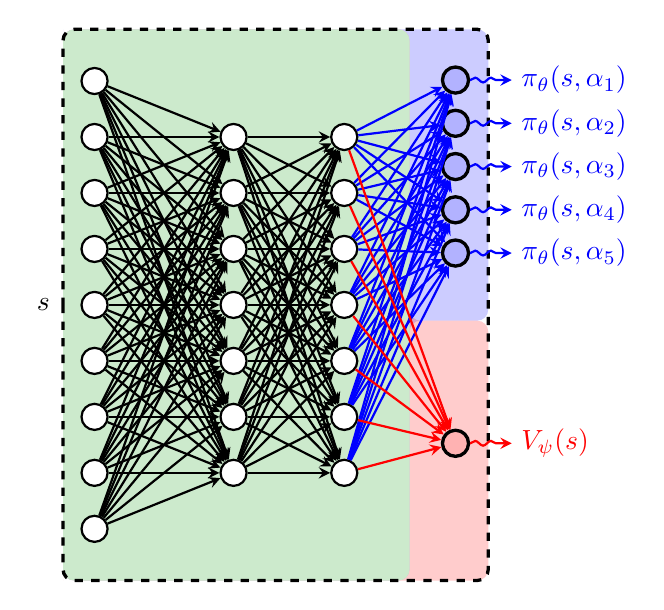
\begin{tikzpicture}

	% boxes
	\path[rounded corners, fill=blue, fill opacity=0.2] (-0.4, 3.5) --  (-0.4, -3.5) -- (4, -3.5) -- (4, -0.2) -- (5, -0.2) -- (5, 3.5) -- (-0.4, 3.5) -- (-0.4, 0);
	\path[rounded corners, fill=red, fill opacity=0.2] (-0.4, -3.5) --  (-0.4, 3.5) -- (4, 3.5) -- (4, -0.2) -- (5, -0.2) -- (5, -3.5) -- (-0.4, -3.5) -- (-0.4, 0);
	\path[rounded corners, fill=white] (-0.4, 0) -- (-0.4, -3.5) -- (4, -3.5) -- (4, 3.5) -- (-0.4, 3.5) -- (-0.4, 0);
	\path[rounded corners, fill=olivegreen, fill opacity=0.2] (-0.4, 0) -- (-0.4, -3.5) -- (4, -3.5) -- (4, 3.5) -- (-0.4, 3.5) -- (-0.4, 0);
	\path [draw, dashed, very thick, rectangle, rounded corners] (-0.4, 0) -- (-0.4, -3.5) -- (5, -3.5) -- (5, 3.5) -- (-0.4, 3.5) -- (-0.4, 0);
	
	% add input nodes
	\node[circle, thick, fill=white, draw] (x1) {};
	\node[circle, thick, draw, fill=white, below=1em of x1] (x2) {};
	\node[circle, thick, fill=white, draw, below=1em of x2] (x3) {};
	\node[circle, thick, fill=white, draw, below=1em of x3] (x4) {};
	\node[circle, thick, fill=white, draw, below=1em of x4] (x5) {};
	\node[circle, thick, fill=white, draw, above=1em of x1] (x6) {};
	\node[circle, thick, fill=white, draw, above=1em of x6] (x7) {};
	\node[circle, thick, fill=white, draw, above=1em of x7] (x8) {};
	\node[circle, thick, fill=white, draw, above=1em of x8] (x9) {};

	% add 2nd layer
	\node[circle, thick, right=4em of x1, fill=white, draw] (xhh1) {};
	\node[circle, thick, draw, fill=white, below=1em of xhh1] (xhh2) {};
	\node[circle, thick, fill=white, draw, below=1em of xhh2] (xhh3) {};
	\node[circle, thick, fill=white, draw, below=1em of xhh3] (xhh4) {};
	\node[circle, thick, fill=white, draw, above=1em of xhh1] (xhh5) {};
	\node[circle, thick, fill=white, draw, above=1em of xhh5] (xhh6) {};
	\node[circle, thick, fill=white, draw, above=1em of xhh6] (xhh7) {};
	
	% 3rd layer
	\node[circle, thick, right=8em of x1, fill=white, draw] (xh1) {};
	\node[circle, thick, draw, fill=white, below=1em of xh1] (xh2) {};
	\node[circle, thick, fill=white, draw, below=1em of xh2] (xh3) {};
	\node[circle, thick, fill=white, draw, below=1em of xh3] (xh4) {};
	\node[circle, thick, fill=white, draw, above=1em of xh1] (xh5) {};
	\node[circle, thick, fill=white, draw, above=1em of xh5] (xh6) {};
	\node[circle, thick, fill=white, draw, above=1em of xh6] (xh7) {};

	% output layer
	\node[circle, very thick, fill=blue!30, draw, right=12em of x1, yshift=5em] (hm1) {};
	\node[circle, very thick, draw, fill=blue!30, below=0.5em of hm1] (hm2) {};
	\node[circle, very thick, draw, fill=blue!30, below=0.5em of hm2] (hm3) {};
	\node[circle, very thick, draw, fill=blue!30, above=0.5em of hm1] (hm4) {};
	\node[circle, very thick, draw, fill=blue!30, above=0.5em of hm4] (hm5) {};
	\node[circle, very thick, fill=red!30, draw, right=12em of x1, yshift=-5em] (hs1) {};

	% add labels for output layer
	\node[right=1.5em of hm1, blue] (mu1) {$\pi_\theta(s, \alpha_3)$};
	\node[right=1.5em of hm2, blue] (mu2) {$\pi_\theta(s, \alpha_4)$};
	\node[right=1.5em of hm3, blue] (mu3) {$\pi_\theta(s, \alpha_5)$};
	\node[right=1.5em of hm4, blue] (mu4) {$\pi_\theta(s, \alpha_2)$};
	\node[right=1.5em of hm5, blue] (mu5) {$\pi_\theta(s, \alpha_1)$};
	\node[right=1.5em of hs1, red] (s1) {$V_\psi(s)$};

	% arrows between input layer and 2nd layer
	\foreach \x in {1,...,9}
	\foreach \y in {1,...,7}
	\draw[-stealth, thick] (x\x) -- (xhh\y);

	% arrows between 2nd layer and 3rd layer
	\foreach \x in {1,...,7}
	\foreach \y in {1,...,7}
	\draw[-stealth, thick] (xhh\x) -- (xh\y);
	
	% arrows between 3rd layer and upper output layer
	\foreach \x in {1,...,7}
	\foreach \y in {1,...,5}
	\draw[-stealth, thick, blue] (xh\x) -- (hm\y);
	
	% arrows between 3rd layer and lower output layer
	\foreach \x in {1,...,7}
	\draw[-stealth, thick, red] (xh\x) -- (hs1);
	
	% decorated arrows for main output variable
	\draw[-stealth, decoration={snake, pre length=0.01mm, segment length=2mm, amplitude=0.3mm, post length=1.5mm}, decorate, thick, red] (hs1) -- (s1);
	
	% decorated arrows between upper output nodes and labels
	\foreach \x in {1,...,5}
	\draw[-stealth, decoration={snake, pre length=0.01mm, segment length=2mm, amplitude=0.3mm, post length=1.5mm}, decorate, thick, blue] (hm\x) -- (mu\x);

	% label for the whole network
	\node[left=0.75em of x1] (l1) {$s$};

\end{tikzpicture}
\end{document}